\documentclass[10pt]{article}
\usepackage[a4paper,margin=18mm]{geometry}
\usepackage{graphicx,hyperref,amsmath}
\hypersetup{colorlinks=true,urlcolor=blue}
\setlength{\parindent}{0pt}
\setlength{\parskip}{6pt}
\begin{document}
\begin{center}\Large Curve25519 torus/S4: native Rust qualification\\[3pt]\normalsize 15 November 2026 -- producer evidence, PCC unverified\end{center}
The reusable Rust crate in \texttt{crypto/tools/torus-s4} compiles the compact
Chebyshev membership circuit and Edwards-y S4 relation over the actual field
$p=2^{255}-19$, $A=486662$. Its consumer in \texttt{cryptanalysis} freezes an
immutable qualifier binary, hashes inputs before compilation, and checks known
triples separately after serializing solver inputs.

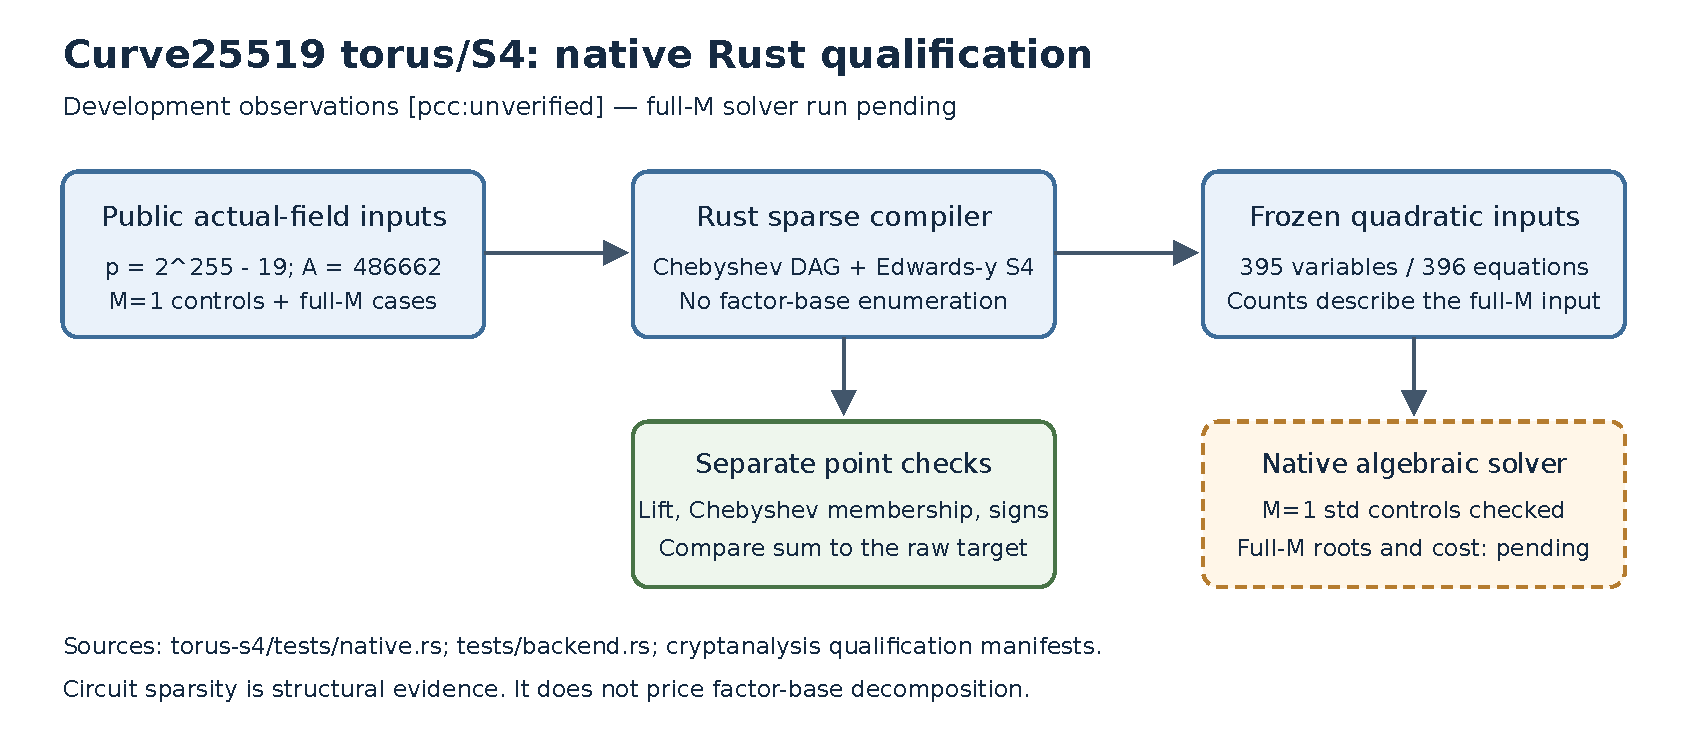
\includegraphics[width=\linewidth]{pipeline.pdf}

\textbf{Observed development controls [pcc:unverified].}
Six native arithmetic/circuit tests pass in the producer log: every coefficient
and variable/equation order matches three frozen historical serializers
($M=5,25,79$); an actual-field planted witness satisfies every input equation,
and separate affine arithmetic checks the signed point sum and recorded
cofactor-cleared target. Mutation and exceptional-input controls are included.
The optional native Singular test reports the expected nonunit/unit basis
classification for the planted/nonmember $M=1$ controls. These are not signed
independent verification or checked absence certificates.

The five-case consumer qualification contains two $M=1$ functional controls
(17 variables, 18 equations) and three cases at
$M=25606137078333158825$ (395 variables, 396 quadratic equations). Known triples
are checks, not inputs to the compiler. Uniform cases have no asserted absence
result. No full-$M$ solver measurement or root recovery is included.

\textbf{Assumptions and remaining work.}
The rational chart excludes zero denominators; recovered roots still require
rational point lifts, Chebyshev membership and sign verification. The pilot
works on raw points before cofactor clearing, with one torus coset. Full-$M$
root extraction, yield and scaling remain pending. The workspace has no EKS
client or live cost readback, and the inspected GitHub image supports ecbench,
not this custom Singular command. The isolated experiment is not substituted
by a local timing run or an integration fixture.

\textbf{Evidence and sources.}
See each study README for raw release-test logs, native backend inputs and
outputs, qualification pre-call/post-call manifests and PCC records
(initial native tests: PCC-20261115-29168c; backend: PCC-20261115-1f2703;
consumer: PCC-20261115-9d157e). All standing remains unverified.
Parameters: \href{https://www.rfc-editor.org/rfc/rfc7748}{RFC 7748}; map conventions:
\href{https://www.rfc-editor.org/rfc/rfc9380}{RFC 9380}; decomposition context:
\href{https://people.maths.ox.ac.uk/petit/files/16PKC_primeECDLP.pdf}{Petit--Kosters--Messeng (2016)}.
The route criteria distinguish static certificate bounds from general solving
cost, and distinguish a resource-limit failure from a proof of route exclusion.
No canonical leaderboard or progress graph is changed by these development checks.
\end{document}
